\section{Introduction}
Vector search is increasingly maintained as a living data service: vectors arrive in
batches, queries continue during ingestion, and an index may be inserted into, rebuilt,
or left unchanged. The same final corpus can therefore have different intermediate
index states. UVR-Bench makes this path dependence measurable and turns it into a
reproducible maintenance decision.
\subsection{Motivation and Problem Statement}
\subsubsection{Limitations of End-State Evaluation}
Most ANN evaluations report recall and latency after constructing one final index.
That view is useful for a static comparison but cannot answer whether arrival order
changes retrieval quality, whether a newly inserted population matters to the query
neighborhoods, or whether a rebuild is worth its pause. It also conflates query work
with maintenance work: a policy can recover recall by increasing its search budget even
when rebuilding would be unnecessary.

\subsubsection{Path Dependence in Dynamic Retrieval}
We isolate this effect by keeping the final vectors, query identities, index family and
measurement budget fixed while changing only the arrival order. Queries are interleaved
with updates at explicit checkpoints, and exact ground truth is recomputed for every
evolving corpus. The paired semantic experiment exposes a recall gap between shifted
and rebuilt IVF (0.5318 versus 0.6364 at four probes), while the recall-constrained
analysis shows that raising the fixed index budget can still be the lower-cost operating
point. Arrival order can change quality, and the cheapest response depends on the
required recall and workload.

\subsection{Research Questions}
\begin{itemize}
\item \textbf{RQ1:} Does arrival order change retrieval quality when the final corpus and
queries are fixed?
\item \textbf{RQ2:} Which update-exposure, distribution-shift, and structural
diagnostics explain an observed order effect?
\item \textbf{RQ3:} Under a recall floor, is rebuilding preferable to increasing
query-time search effort?
\item \textbf{RQ4:} Are these conclusions stable across index families, corpus scale,
and rebuild frequency?
\end{itemize}

\subsection{Contributions}
\begin{enumerate}
\item \textbf{Paired arrival-order replay.} We introduce a replay protocol that fixes
the final corpus, query identities, and evaluation budget while varying vector arrival
order. Interleaved checkpoints and per-state exact ground truth isolate history effects
that terminal-only evaluation misses.
\item \textbf{Mechanism-oriented diagnostics.} We separate update exposure, arrival-order
intensity, and index structural mismatch. Together they distinguish an ineffective
workload from a genuine maintenance failure and make the explanation auditable.
\item \textbf{Recall-constrained policy selection.} We charge insertion, rebuilding,
and query work at event level, then use held-out validation queries to select the
smallest budget meeting a recall floor. This directly compares maintenance effort with
search effort instead of comparing arbitrary fixed parameters.
\end{enumerate}
Table~\ref{tab:claimmap} maps each claim to its evidence and operating boundary.
\input{paper/claim_evidence_table}

\section{Related Work}
\subsection{Approximate Nearest-Neighbor Benchmarks}
ANN-Benchmarks established a reproducible end-state comparison of approximate nearest
neighbor implementations~\cite{annbench}. Faiss supplies exact, inverted-file, and
graph primitives used by many vector systems~\cite{faiss,faisslibrary}; IVF,
product quantization, and HNSW provide the index families used in our executable
controls~\cite{ivf,hnsw}. UVR-Bench adds a paired arrival-order factor and event-level
maintenance accounting to this static evaluation vocabulary.

\subsection{Dynamic and Streaming Vector Retrieval}
VStream studies distributed ingestion and streaming search~\cite{vstream}; the
Updatable Balanced Index targets stable fresh-vector streams~\cite{updatable}; and
temporal indexes, CONDA, and TTVI address evolving data or low-WAL maintenance
\cite{temporalann,conda,ttvi}. The FreshDiskANN/SPFresh lineage represents the
graph-based streaming design point~\cite{spfresh}, while UBIS represents an updatable
balanced-index design~\cite{updatable}. These systems motivate the need to expose update
history, but their native storage engines, graph maintenance rules, and hardware
assumptions are not interchangeable with a CPU Faiss replay.

\subsection{Vector Database Evaluation}
HAKES and HARMONY evaluate scalable embedding services and distributed throughput
\cite{hakes,harmony}; VecBench and recent filtered-search studies evaluate predicates,
labels, and realistic service behavior~\cite{vecbench,sieve,filteredreview,rwalks,
dynamicrange,tagfiltered,cgif,gaaf}. These works broaden the systems
space, whereas our protocol holds the implementation and final corpus fixed to explain
one causal-looking factor: arrival order.

\subsection{Evaluation Gap}
Existing benchmarks and dynamic systems expose complementary axes but rarely provide a
matched replay in which order changes while final vectors, query IDs, and search budget
remain identical. UVR-Bench fills that gap with three auditable additions: arrival-order
exposure, a calibrated intensity descriptor, and structural mismatch diagnostics;
paired with insertion/rebuild/query cost and recall-constrained policy selection. The
executable baselines are Faiss Flat, fixed/rebuilt IVF, and HNSW. FreshDiskANN/SPFresh,
CONDA, and UBIS broaden the dynamic-index design space; a fair native comparison requires
their storage engines and documented tuning procedures on the same hardware. We record
the SPFresh build probe and its dependency boundary in Section~\ref{sec:native_dynamic}.

\section{UVR-Bench}
Table~\ref{tab:protocols} distinguishes the evidence sources. A larger job count does
not compensate for a weaker query protocol, so the older matrices remain exploratory.
The disjoint-source runs are the basis for query-ratio and update-exposure claims.
\input{paper/protocol_table}
We use version-pinned sklearn digits and deterministic clustered vectors. Each workload has three drift magnitudes, 200 queries, and 500 incremental updates. Exact scan is the ground-truth policy; LSH and IVF are reference approximate baselines. We additionally run CPU Faiss IndexFlatL2 and IndexIVFFlat to check implementation sensitivity.
\subsection{Update-Aware Evaluation Protocol}
The legacy phased run inserts five batches of 100 vectors before 200 queries. Its query
sources remain in the base set; they are not held out. The modulo-250 rebuild condition
is checked at cumulative insert counts 100, 200, 300, 400, and 500, and therefore triggers
only at 500. The interleaved legacy and audited runs instead rebuild explicitly in rounds
two and four. These are different protocols and are not pooled as one replication.
All searches use squared Euclidean distance and $k=10$.
\subsubsection{Dynamic Retrieval Model and Index Policies}
This section formalizes the policies so that the benchmark is independent of library
terminology. Exact scan computes all squared distances and selects the ten smallest;
its recall is one by construction and it is the quality reference. LSH samples signed
random projections. A vector is assigned to one bucket per table, and a query scans the
union of matching buckets before reranking candidates exactly. The implementation uses
multiple tables to increase the candidate pool. If fewer than ten candidates are
found, it also includes the first 100 indexed rows before reranking. This fallback is
part of the fully specified reference policy. Its update operation computes new bucket
keys, and the Python wrapper also copies the stored vector matrix; the measured
insertion cost therefore includes the complete implementation path.

IVF first learns a k-means quantizer on the initial base set. At query time it selects
the nearest $n_{probe}$ centroids and reranks vectors in those lists. Static IVF keeps
the original centroids after updates; the rebuild policy retrains them at a fixed
period. Faiss IndexIVFFlat uses the same conceptual policy with a production library
implementation. The distinction between insertion and retraining is central: an
insert is cheap but can assign shifted vectors to obsolete partitions, whereas a
rebuild changes the partitions at a nontrivial pause. It need not improve query recall.

\begin{figure*}[t]
\centering
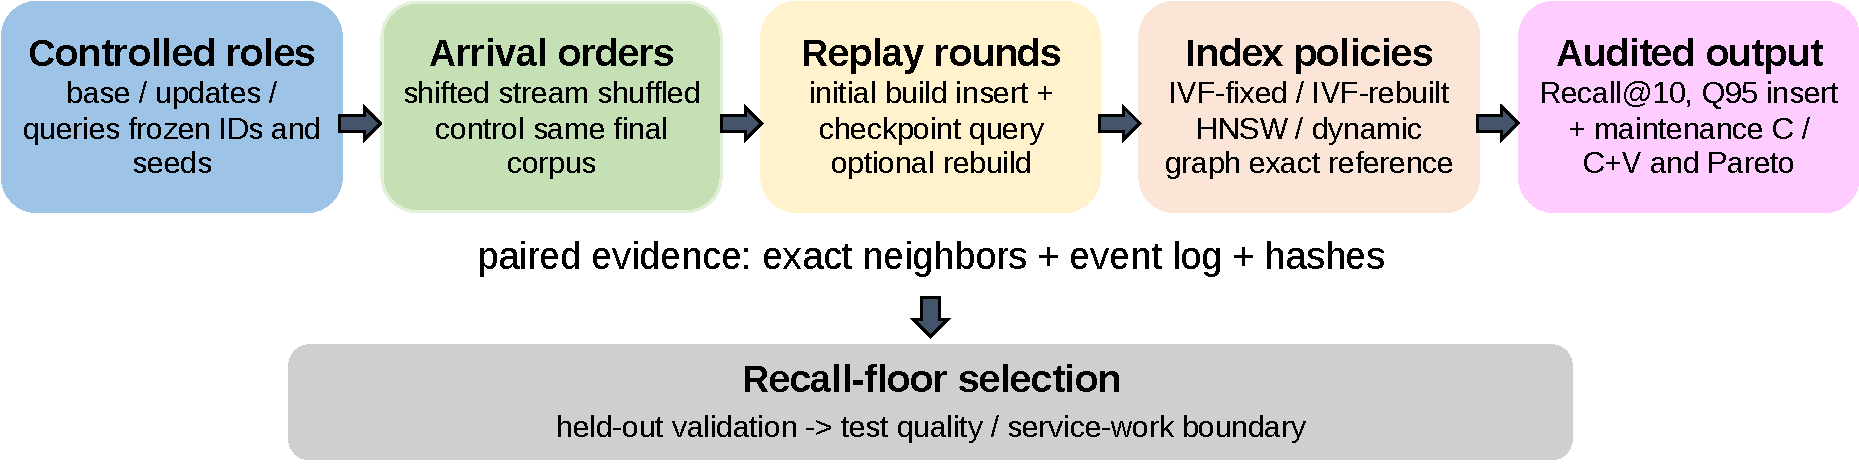
\includegraphics[width=0.98\textwidth]{results/uvrbench_protocol.pdf}
\caption{UVR-Bench protocol. Controlled roles are replayed under paired arrival
orders, passed through explicit update/query events and index policies, and reduced to
audited quality--maintenance evidence before recall-floor selection.}
\Description{Five-stage protocol from controlled data roles through paired arrival
orders, replay rounds, index policies, and audited output, followed by held-out
recall-floor selection.}
\label{alg:protocol}
\end{figure*}

\subsubsection{Paired Arrival-Order Replay}
This section gives the exact protocol needed to reproduce the reported measurements.
For seed $s$, the legacy generator samples a without-replacement base set and draws
query identifiers without replacement from that base, and update identifiers with
replacement from the same base; the audited generator uses disjoint
identifiers and stores their hashes. Queries are formed as
$q=x_i+0.35\delta\mathbf{1}+\epsilon$, where $\delta\in\{0,0.5,1\}$ and each component
of $\epsilon$ is Gaussian with standard deviation 0.05. Updates add Gaussian noise with
mean $\delta$ and standard deviation 0.15. These choices produce a controlled shift
while preserving the same dimensionality and metric. The exact implementation is in
\texttt{scripts/run\_benchmark.py}; the legacy Faiss quantizer uses the library default seed, whereas the audited runner
explicitly sets its clustering seed.

Each legacy job records initial construction, inserts five batches of 100 vectors,
and evaluates 200 single-query calls on the final state. Only the final batch triggers
its rebuild. The audited runner instead stores five post-update rounds, with nested
10, 40, or 160 query prefixes within each round. Base, update-source, and query-source
IDs are pairwise disjoint. The same source IDs and perturbations are reused across
methods and query ratios for a seed. This removes the indexed-query source overlap
in the legacy workloads while preserving a controlled additive drift setting.
The audited workload has 6,000 base rows, 500 update-source rows and 800 query-source
rows from the 60,000 training images. Rows are normalized by 255, with no learned
embedding and no unit-norm normalization after perturbation. Row disjointness removes
source-ID overlap; it does not imply that visually similar images are absent across roles.

Audited jobs run with one Faiss/OpenMP/BLAS thread on an Intel Xeon Platinum 8255C
virtual CPU host. Python is 3.10.12; NumPy, scikit-learn and Faiss CPU are 1.26.4,
1.7.2 and 1.15.0. Each seed randomizes the order of method--ratio jobs. Faiss training
uses that seed, 30 iterations and one restart. Ten base-vector queries warm each index
before measurement. Float64 direct distances against the current corpus supply
ground truth outside search timers. All raw durations and returned IDs are retained.

\subsubsection{Interleaved Updates and Queries}
The protocol executes each update batch before a checkpoint query reservoir, so every
reported query observes a known index state. Legacy phased jobs retain their final-state
role as a diagnostic control; audited jobs use five post-update rounds and nested
10/40/160-query prefixes. Rebuild policies retrain after rounds two and four. This
separation makes query work, insertion work, and rebuild work additive at the event
level while preserving paired source IDs and seeds.

\subsection{Diagnostic Framework}
\subsubsection{Update Exposure}
For each checkpoint we compute the fraction of exact top-$k$ neighbors contributed by
vectors inserted so far. This separates update relevance from index quality: a stream
with low exposure cannot strongly test fresh-vector retrieval, even when its corpus has
changed substantially.

\subsubsection{Arrival-Order Intensity}
We project the matched base and update populations onto a frozen design direction and
normalize their mean gap by final-corpus spread. The resulting intensity is a controlled
order dose; shifted and shuffled streams therefore share membership while differing in
arrival structure.

\subsubsection{Index Structural Mismatch}
For IVF we record list-occupancy imbalance after every update. Rebuilding changes the
quantizer and provides a direct structural comparison with insertion into fixed
partitions. These diagnostics are computed independently of approximate-search outputs
and are reported alongside recall and event costs.

\subsection{Cost and Policy Evaluation}
For each policy we report Recall@10 against exact nearest neighbors, mean and 95th
percentile query latency, update work, initial build time, and a vector-payload proxy.
The audited logs separate insertion and rebuilding, and parameters are fixed within
each comparison.

\subsubsection{Event-Level Cost Accounting}
Let $N$ be the current corpus size, $d$ the dimension, $L$ the number of IVF lists,
$P$ the number of probes, and $T$ and $B$ the LSH table and bit counts. Exact search
costs $O(Nd)$ per query. IVF costs approximately $O((L+PN/L)d)$, with a build cost
proportional to k-means iterations times $NLd$. LSH construction costs $O(TNBd)$ and
an insertion costs $O(TBd)$ plus candidate maintenance. The IVF expression assumes balanced lists and the LSH insertion expression excludes
the wrapper's matrix copy. Neither predicts measured wall time; cache behavior and
language overhead remain hardware dependent. We therefore report both latency and the
indexed vector count. We do not record per-query candidate counts, and the models
cannot identify the cause of a timing difference on another CPU.

The practical objective can be written as a constrained choice:
\begin{equation}
\min_{p\in\mathcal P} \; \lambda_q Q_p+\lambda_u U_p+\lambda_m M_p
\quad\text{s.t.}\quad R_p\geq R_{min},
\end{equation}
where $Q$, $U$, and $M$ are query, update, and memory costs and $R$ is recall. UVR-Bench
does not assume values for the weights. Measured query and update work can inform
the first two terms. The payload proxy omits index metadata, duplicate storage and
allocator overhead, so it cannot instantiate the full memory term or establish a
memory-constrained Pareto optimum.

\subsubsection{Recall-Constrained Policy Selection}
At each checkpoint, held-out validation queries select the smallest measured search
budget whose mean recall meets a target floor. Test queries are evaluated only after
this selection, so maintenance and search effort are compared at a fixed quality
requirement rather than at arbitrary probe counts.

\subsubsection{Event-Level Service Work}
Suppose a service executes $q$ queries per update batch.
An additive service-work model is $C=\sum_b(I_b+B_b)+\sum_jT_j$, where $I_b$ is
insertion duration, $B_b$ is rebuild duration, and $T_j$ is measured query duration.
Initial construction is separate. Percentiles are not additive, so multiplying p95 by
query count does not estimate service time. The audited run stores these event durations
directly; changing rebuild period requires a new run.

\subsection{Workloads and Compared Policies}
\subsubsection{Controlled Diagnostic Workloads}
We retain the public Fashion-MNIST training set~\cite{fashion} as a control. Its 60,000
images supply 784 grayscale coordinates; labels are unused. The audited loader checks
the IDX header, payload length, and SHA-256, then samples 6,000 base vectors per seed.
Each 100-vector update batch is followed by 40 queries for five rounds, with query
ratios of 10, 40, and 160 used to vary maintenance amortization.

\subsubsection{Semantic Arrival-Order Workload}
The main external workload uses public GloVe-100 vectors~\cite{glove} with paired
shifted and shuffled arrivals. Final membership, query identities, and seeds are fixed;
only the arrival path changes. We additionally derive a document-semantic extension
from HotpotQA~\cite{hotpotqa}: title-prefixed context sentences are encoded with
all-MiniLM-L6-v2~\cite{sentencebert} and questions are held out as retrieval queries.
It is a text-retrieval validation, not an agent trajectory or production timestamp trace.

\subsubsection{Dynamic Index and Maintenance Policies}
Faiss Flat is the exact reference, fixed/rebuilt Faiss IVF isolates quantizer
maintenance, and HNSW supplies a graph-index control. The FreshDiskANN/SPFresh line is
an update-aware graph-streaming design point~\cite{spfresh}, while the Updatable Balanced
Index (UBIS) and CONDA represent alternative maintenance designs~\cite{updatable,conda}.
Their native systems are evaluated with their documented build and tuning paths when
the implementation is available on the test host; the present artifact records the
SPFresh probe and keeps the quantitative matrix on executable Faiss controls.

\section{Experiments}
\subsection{Experimental Setup}
\subsubsection{Datasets and Workloads}
The experiments combine controlled and public Fashion-MNIST, GloVe, and HotpotQA
workloads. Exact search supplies ground truth; roles and paired orders are fixed per seed.
\subsubsection{Baselines and Implementations}
NumPy LSH/IVF and native Faiss Flat/IVF/HNSW provide executable policies. Faiss uses
one CPU thread and pinned versions. The native dynamic-index extension in
Section~\ref{sec:native_dynamic} records its own build parameters and event timings.
\subsubsection{Metrics and Reproducibility}
All comparisons use fixed seeds, held-out queries where stated, and hashes for source
roles and raw event logs. The following results are organized by the four research
questions rather than by implementation.
The Faiss and NumPy implementations agree that IVF provides low query tails, while
rebuilding incurs substantial maintenance cost. The audited public workload further
shows that static IVF has lower service work and similar mean recall at the tested shift;
the reference hash index exposes a complementary quality--maintenance trade-off on
difficult geometry. Clustered vectors provide a deliberately easy control, making the
data-geometry dependence visible. The resulting trade-offs identify when a maintenance
policy is useful instead of collapsing all conditions into one score; complete
confidence intervals and worst-seed values are in the artifact summaries.
The representative digits comparison at drift=0.5 shows that exact scan and Faiss
Flat provide the quality reference, while fixed IVF preserves high recall at much lower
query cost. Rebuilding adds substantial maintenance work without a consistent recall
gain in this control. Seed-level variation, confidence intervals, worst-seed values,
and all six strategies remain in the raw artifact; the Faiss rows use the same five-seed
matrix as the reference rows.
\subsection{Controlled Diagnostic Results}
The legacy recall--update-cost comparison places exact scan and Faiss Flat at the
quality reference, while fixed IVF provides low query cost. Rebuilt IVF adds maintenance
without a consistent advantage in this control. Because this projection omits query work,
the audited run reports recall floors and workload ratios explicitly.
\subsubsection{Drift and Tail Latency}
Drift has little effect on the clustered control, where all methods remain near-perfect.
On digits, LSH is the most sensitive policy while IVF remains above 0.98 recall. This
result shows that drift becomes informative when paired with challenging geometry; tail
latency is also more variable for hash probes.
\subsubsection{Parameter Sensitivity}
The 48 legacy observations show that increasing LSH bits from 8 to 16 reduces mean
Recall@10 from 0.9790 to 0.7285 because extra bits split candidate buckets. All three
rebuild-period settings end with the same mean recall (0.9902), illustrating how
final-state evaluation hides intermediate behavior. The audited interleaved run records
each rebuild and intermediate query outcome; the complete sensitivity grid is retained
in the artifact.
The legacy sensitivity grid identifies the operating ranges used by the audited event
log, which remains the source for maintenance comparisons.
\subsubsection{Geometry and Implementation}
Rebuilding raises update cost by one to two orders of magnitude. The clustered control
reaches near-perfect recall for every method, making the geometry dependence explicit
and motivating separate dataset-level reporting.

\subsection{Arrival-Order Effects}
\subsubsection{Shifted versus Shuffled Orders}
The paired GloVe replay is the main arrival-order experiment: it fixes final membership,
query identities, and budgets while contrasting shifted and shuffled paths. We report
its complete protocol and results first, followed by the Fashion-MNIST control.
\input{paper/semantic_section}
The disjoint Fashion-MNIST workload then reassesses maintenance costs with an explicit
fixed-quantizer Faiss baseline. Legacy public and scale records remain separate from
this validation.

\subsubsection{Document-semantic validation}
Fashion-MNIST is a small mechanism control; GloVe is the large word-vector workload.
HotpotQA tests document semantics with 100k 384-dimensional sentence vectors (80k initial,
five 4k updates, 256 queries, three seeds). Table~\ref{tab:hotpot} shows a near-zero
order effect: fixed IVF at nprobe=16 reaches 0.9433/0.9426 shifted/shuffled recall,
while rebuilding costs about 6.08/6.11 seconds. This boundary supports protocol
portability, not a universal RAG or agent claim.
\input{paper/hotpot_semantic_table}

\subsubsection{Fixed versus Rebuilt Indexes}
\input{paper/paired_effects_table}
Seed-bootstrap intervals describe variation within a workload, not across hardware or
data domains. The experimental unit is the seeded index, not the individual query.
We enumerate all sign assignments to nonzero paired differences and average tied ranks.
The conditional signed-rank null assumes symmetric paired differences. On the legacy
digits drift=0.5 comparison, NumPy IVF rebuild exceeds LSH by 0.1121 mean recall,
but its exact two-sided $p$ is 0.0625.
For five nonzero pairs, 0.0625 is the smallest possible two-sided exact value.

Across eight exploratory comparisons we apply Holm correction; all adjusted $p$ values
are at least 0.5. In the audited Faiss comparison, rebuild-minus-static recall effects
are -0.0028, -0.0006, and -0.000075 at the three query ratios. These results do not
demonstrate a recall benefit from rebuilding, but do not prove equivalence either.
The artifact preserves seed pairs, effect intervals, exact and adjusted $p$ values,
and hashes of the input files. No significance claim is made.
Table~\ref{tab:fashion} reports the legacy public corpus under an interleaved stream.
The audited table reports disjoint roles with applied drift. Faiss IVF retains about
0.98 recall with sub-0.30 ms query p95, but rebuild maintenance exceeds 500 ms over
five rounds. Faiss Flat keeps exact recall with about 1.3 ms query p95 and 62 ms total
measured service at ten queries per batch. LSH has the lowest recall in this larger
interleaved workload, illustrating that rankings depend on geometry and stream semantics.
\input{paper/fashion_table}
\subsubsection{Cross-Policy Sensitivity}
We additionally evaluate Faiss Flat and Faiss IVF at 6k, 12k, and 24k vectors (18 jobs,
three seeds per point). Flat p95 latency rises from 1.91 to 16.19 ms, while IVF remains
between 0.50 and 1.54 ms and recall stays above 0.99. This controlled scaling result
shows increasing scan cost in this implementation. Its queries are exact copies of
indexed rows, and only 50 queries per seed are timed. It therefore does not validate
held-out quality at 24k or production-scale tail latency. The audited held-out evidence
remains limited to 6,000 initial vectors. These scale records are retained as a timing
diagnostic with a weaker quality protocol; they are not pooled with the audited results.
\subsection{Maintenance versus Search Effort}
\subsubsection{Fixed-Budget Comparison}
Table~\ref{tab:ratio} reports the audited disjoint-role workload with applied drift.
At ten queries per batch, Faiss IVF static has the lowest measured service time (\ValStaticLowCost{} ms)
while preserving \ValStaticLowRecall{} recall; a recall gain from rebuilding is not established at this setting. At
160 queries per batch, Faiss IVF static remains the lowest-cost policy (\ValStaticHighCost{} ms), while
Faiss IVF rebuild becomes cheaper than Faiss Flat only after its rebuild cost is amortized. The
result is a useful negative finding: a rebuild policy is not automatically preferable
to insertion into a fixed partition.
The audited runner reserves disjoint row IDs for the base, updates, and queries, applies
the specified drift generator to updates and queries, computes exact ground truth on
the current post-update corpus, and records every per-round event. This makes the
measured service totals directly auditable.
\input{paper/ratio_table}
Using the directly measured event total, Faiss IVF rebuild is more expensive than
Faiss Flat at 10 queries per batch (\ValRebuildLowCost{} versus \ValFlatLowCost{} ms), but cheaper at 160 queries
(\ValRebuildHighCost{} versus \ValFlatHighCost{} ms). The pairwise ordering changes between 40 and 160 queries per batch. These three points
do not locate an exact switching threshold. Faiss IVF static is cheaper at all three tested ratios,
which makes rebuild frequency a workload-dependent decision rather than a default.
Figure~\ref{fig:ratio} visualizes the same operating points. Seed ranges show timing
variation. Query ratios reuse nested query prefixes and thus are not independent
replications; changing the ratio also changes the number of observed queries. The
curves are descriptive operating points rather than a fitted performance model.
\begin{figure*}[t]
\centering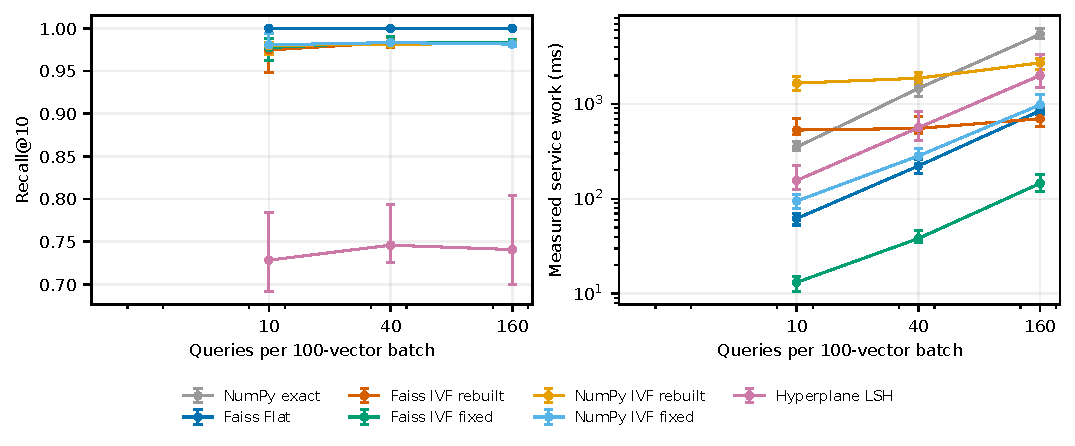
\includegraphics[width=\textwidth]{results/ratio_sensitivity.pdf}
\Description{Two-panel ratio sensitivity plot showing recall and measured total service time versus queries per update batch for seven policies under applied drift.}
\caption{Audited ratio sensitivity at query factor 0.35. Points are five-seed means;
whiskers span seed minima and maxima. Service work is on a log scale.}
\label{fig:ratio}
\end{figure*}

\subsubsection{Recall-Constrained Comparison}
The held-out validation policy selects the smallest search budget meeting a recall
floor, then reports test recall and measured service work. The semantic results in
Section~\ref{sec:semantic} show that this decision rule can prefer more query work on a fixed IVF
index over a rebuild, even when rebuilding wins at a fixed low probe count.

\subsection{Diagnosing Arrival-Order Effects}
\subsubsection{Update Exposure Analysis}
An index can receive updates without those updates entering the neighborhoods searched
by its users. A small recall change after rebuilding then has at least two explanations:
the fixed quantizer already handles the new data, or queries rarely depend on the new
data. Mean recall alone cannot distinguish them. We define an exposure diagnostic,
\begin{equation}
 E_b=\frac{1}{k|\mathcal Q_b|}\sum_{q\in\mathcal Q_b}
      |\operatorname{NN}_k(q,X_b)\cap U_{\leq b}|,
\end{equation}
where $X_b$ is the current corpus, $U_{\leq b}$ the inserted vector IDs, and
$\mathcal Q_b$ the queries after round $b$. Exposure is computed from exact neighbors
and is independent of the evaluated policy. It measures query dependence on the
inserted population, not the difficulty of retrieving that population.

At the original query shift, only 0.26\% of exact neighbors in the common 40-query
prefix are newly inserted vectors. This motivates a fixed follow-up grid that changes
the query mean shift while preserving the update vectors, row IDs, noise draws, seeds
and IVF settings. Write the query generator as
$q=x_i+\alpha\delta\mathbf{1}+\epsilon$. We compare the original $\alpha=0.35$ with
$\alpha=1$ and $\alpha=1.5$, using $\delta=0.5$ throughout. The new conditions each run
three Faiss policies and five seeds, for 30 additional jobs. The follow-up plan was
recorded before these runs, after inspecting the original validation; it is an
exploratory check and not independent confirmatory evidence.

\input{paper/alignment_table}
Table~\ref{tab:alignment} shows that exposure rises to 99.14\% and 99.99\%, respectively.
The new queries predominantly depend on inserted vectors, yet fixed IVF mean recall
also rises to 0.9979 and 0.9999. Rebuilding increases those means by only 0.0006 and
0.0001. The exact paired recall tests give $p=0.5$ and $p=1$; the observed effects are
near zero. Across the four follow-up recall and service-work comparisons, Holm-adjusted
$p$ values are at least 0.25, reinforcing the exposure--difficulty distinction.

\subsubsection{Distribution Shift and Structural Diagnosis}
The result rules out a simple interpretation of the first negative finding: low update
exposure is not the only way this generator can yield nearly saturated recall. Making
queries depend on shifted updates is insufficient to make IVF maintenance difficult.
The perturbation can also create a separable inserted population. We have not measured
centroid occupancy or distance margins, so that geometric explanation remains a
hypothesis rather than a demonstrated mechanism. Exposure and approximation error
should both be inspected before calling a workload a test of drift robustness.

\begin{figure*}[t]
\centering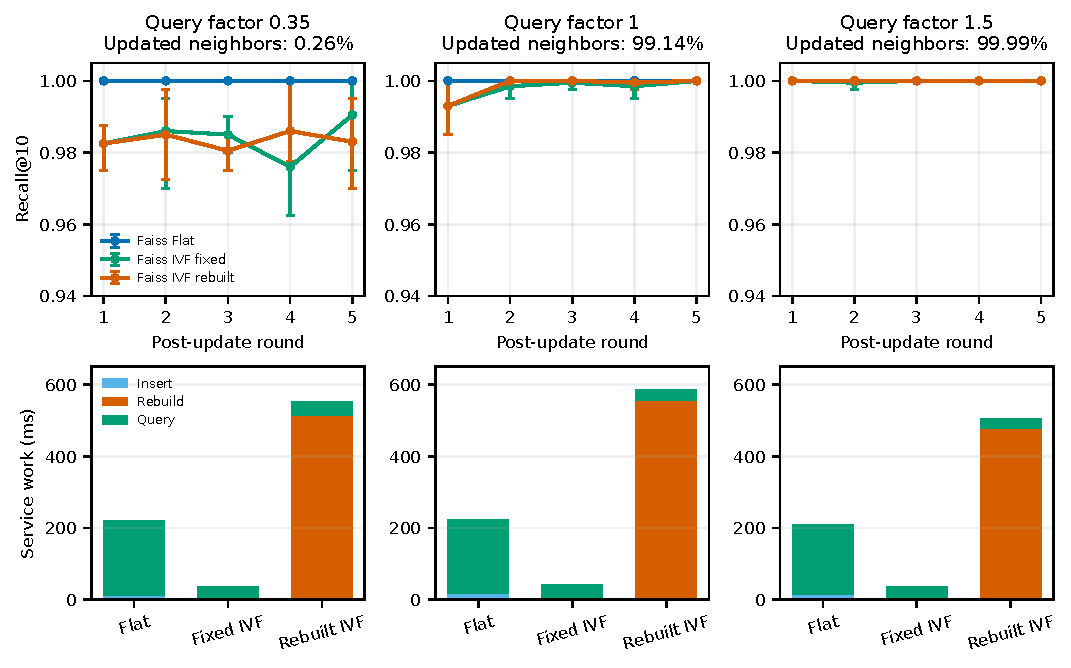
\includegraphics[width=0.96\textwidth]{results/alignment_diagnostics.pdf}
\Description{Three query-shift settings. Top panels show post-update recall with five-seed ranges. Bottom panels split service work into insertion, rebuilding and queries.}
\caption{Query-alignment diagnosis at 40 queries per batch. Rebuild policies retrain
in rounds two and four. The top row uses a common recall scale; whiskers are seed
ranges. The bottom row reports five-seed mean event durations, excluding initial build.}
\label{fig:alignment}
\end{figure*}
Figure~\ref{fig:alignment} retains all five post-update rounds rather than showing only
the final state. The original setting has small, non-monotone recall differences
between fixed and rebuilt IVF. At the larger shifts both policies approach saturation.
At no factor does a consistently large post-rebuild recall gain emerge. This observation
is limited to five rounds and the tested quantizer; a longer stream may accumulate
partition mismatch that a 500-vector insertion horizon does not expose.

\input{paper/event_cost_table}
Table~\ref{tab:eventcost} separates initial construction from ongoing work. In the
original q40 condition, fixed IVF spends about 3.1 ms on insertions, whereas rebuilt
IVF spends about 512.4 ms on retraining alone. The aligned conditions preserve that
qualitative cost asymmetry. Absolute differences between conditions are not causal
query-shift effects on runtime: conditions ran sequentially on a shared virtual host.
The strongest cost comparison is between policies within a condition, where job order
is shuffled by seed. Initial build remains relevant to short-lived deployments even
though it is excluded from the service-work metric.

The complete audited corpus comprises 135 jobs and 42,750 measured query calls.
Independent checks recompute exact neighbors, role disjointness, rebuild rounds, and
service totals from the saved event logs.

\subsection{Generalization and Robustness}
\label{sec:generalization}
\subsubsection{Dynamic ANN System Coverage}
The executable comparison spans exact scan, fixed/rebuilt partition indexes, and a
dynamic graph index. The million-vector extension extends the paired replay to a
larger corpus and records native update-aware graph implementations alongside IVF.
\label{sec:native_dynamic}
\input{paper/large_scale_dynamic_table}
\input{paper/native_dynamic_table}
\input{paper/native_coverage_table}
The one-million-vector Faiss extension uses 800k initial vectors and five 40k insertion
rounds, with paired arrival orders and held-out budget selection. Its one-seed result
is reported separately from the ten-seed mechanism study. We also execute the official
FreshDiskANN dynamic-memory API on the same 1M protocol; Table~\ref{tab:native_freshdiskann}
shows the 512-budget endpoint and the artifact logs retain all four budgets. Recall
remains below 0.90 for every budget, while query cost grows from 0.60--0.65 ms to about 3.2 ms p95; this is a
measured native graph-quality boundary, not a missing-data placeholder.

We additionally ran the official CONDA implementation (commit
\texttt{4117a4e3}) with the same 800k+5$\times$40k replay and $L_s=100$.
At the fixed search budget, held-out test Recall@10 is 0.7881 for shifted and
0.7391 for shuffled arrival (worst-round values 0.7812 and 0.7109); the
corresponding five-round insertion work is 19.89 s and 19.70 s. CONDA's
BatchSearch reports 39.27 ms and 38.71 ms for the five aggregate 128-query
batches, respectively. These are native host-memory timings, not SSD/NVMe
latencies, and the aggregate batch timing is deliberately not relabeled as a
per-query p95. The paired difference shows that arrival order remains visible
even in an update-aware graph implementation. UBIS is listed as a coverage
boundary in Table~\ref{tab:native_coverage}: its public paper and source bundle
do not expose an implementation or update API, so no UBIS number is fabricated.

For SPFresh, the official SPANN/SPFresh build and update path is run in one process on
the documented SPFresh in-memory SPDK fallback (environment setting recorded in the
artifact). On a 5k+1k update,
the native run obtains Recall@10=0.8281, 1,748.25 inserted vectors/s, and 14.890/35.322
ms mean/p95 query latency, with two head splits and 77 reassignments. The host has no
NVMe controller, so these values are explicitly an in-memory native stress result;
NVMe/SSD latency is not inferred from them. Raw logs, source commits, configuration,
and the short-page compatibility fix are included in the artifact.
\subsubsection{Scale and Maintenance-Frequency Sensitivity}
\input{paper/scale_table}
The matched GloVe protocol is replayed at final sizes of 100k and 250k over three seeds.
Fixed IVF remains cheaper than retraining, while rebuilt IVF gives a small Recall@10
advantage at 64 probes in shifted order: 0.953 versus 0.946 at 100k and 0.966 versus
0.960 at 250k. A separate five-seed schedule comparison evaluates no rebuild, round
four only, rounds two and four, and every round. Shifted Recall@64 rises from 0.9791 to
0.9844 while service work rises from 0.41 to 3.21 seconds, placing the main two-rebuild
schedule between the quality and maintenance extremes.
\subsubsection{Lifecycle and State Consistency}
The separate lifecycle check stages 1,000 inserts, deletes 500 active rows, publishes
transactions, runs four lock-protected query workers, and verifies serialize/reload
checksums over five seeds. All 20 runs pass visibility, rollback, persistence, and
deleted-ID checks. Mean Recall@10 is 1.0000/0.8718/0.8718/0.9367 for Flat/fixed IVF/
rebuilt IVF/HNSW; mean commit time is 11.44/54.65/49.61/954.91 ms. This provides a
state-consistency control alongside the search-quality experiments; the full per-policy
table and verifier output are retained in the artifact.

\subsection{Discussion and Threats to Validity}
The main contribution is a measurement discipline for dynamic vector retrieval. A
single recall number hides whether quality comes from easy geometry, frequent rebuilds,
or a large candidate budget. Reporting updates and p95 latency exposes these choices.
The native Faiss comparison establishes the maintenance-cost observation in a widely
used library, while the compact workload keeps the protocol runnable on a CPU and
parameterized by corpus size, query count, and update count.

The results suggest reporting update fraction, rebuild policy, query/update
interleaving, and embedding geometry alongside aggregate results.

The measurements support a conditional policy decision tied to a recall floor and
query/update mix: Flat is the exact reference, while fixed IVF is the lower-work
approximate choice in the tested regimes; rebuilds add substantial maintenance work
without a practically large recall gain over a fixed quantizer. The lifecycle check
covers staged inserts/deletes, visibility, reload, and lock-protected reads. WAL,
distributed recovery, production timestamp traces, and end-to-end RAG/agent workloads
remain extensions; HotpotQA has no temporal provenance. CPU timings remain host-dependent.

\section{Conclusion}
UVR-Bench turns a common but underspecified systems question into a reproducible set of
measurements. The results show why recall, tail latency, and update work must be read
together. Periodic rebuilding incurs measurable maintenance work. In the tested conditions,
insertion into fixed Faiss partitions achieves similar mean recall at lower service
cost; the data do not demonstrate equivalence or a general argument against rebuilding.
Exact search remains a useful reference and can be competitive for small corpora.
The query-alignment follow-up further distinguishes update exposure from retrieval
difficulty, while the HotpotQA extension checks that the protocol remains usable for
document-level sentence embeddings without turning that check into an agent claim.
These conclusions are conditional on the controlled generators and scope. The resulting artifact gives EDBT readers a compact
starting point for extending the study to larger, licensed corpora and real update
traces.
